% \import{..}{wellington-commands.tex}

A robótica móvel está se desenvolvendo rapidamente, no entanto, aplicações 
em ambientes sem uma infraestrutura de mapeamento global exigem técnicas 
de mapeamento e percepção robustas para capacitar agente móveis a 
navegar de maneira autônoma em ambientes complexos \cite{saeedi2016multiple}. Aplicações dessa 
natureza não surgem apenas da exploração de outros planetas onde não há 
GPS, por exemplo. Pelo contrário, há diversos cenários na Terra onde o 
GPS não funciona adequadamente, como debaixo d'água, 
em minas subterrâneas e dentro de construções. Este problema é denominado SLAM e resolvê-lo implica em empoderar soluções de robótica móvel, 
que atuem nesses cenários, com aplicações reais e comerciais.

O problema de Mapeamento e Localização Simultâneos, conhecido pela sigla SLAM por conta do termo em inglês \textit{Simultaneous Localization and Mapping}, pergunta se é possível para um robô móvel ser colocado em um ambiente desconhecido a priori e incrementalmente construir um mapa deste ambiente enquanto simultaneamente se localiza neste mapa. Ou seja, tanto a trajetória da plataforma móvel quanto a localização das características do mapa (também conhecidas por \textit{landmarks}) são estimadas em tempo real sem a necessidade de nenhum conhecimento a priori de suas localizações \cite{durrant2006simultaneous}, ou infra estrutura de localização prévia, como GPS.

SLAM também já foi conhecido como Mapeamento e Localização Concorrentes (CML, do inglês \textit{Concurrent Mapping and Localization}), porém este termo caiu em desuso a partir de 1995 quando o termo SLAM foi cunhando por \citeonline{durrant1996localization} no Simpósio Internacional de Pesquisa em Robótica, ISSR, onde originalmente era chamado \textit{Simultaneous Localization and Map Building}. A solução do problema SLAM é fundamental para atingir a robótica móvel autônoma e independente de operadores \cite{durrant2006simultaneous}. Entretanto resolver o problema de localização e mapeamento simultâneos, apesar de solucionado, não é uma tarefa trivial tanto do ponto de vista teórico como do ponto de vista da implementação \cite{durrant1996localization}.

\subsection*{Caracterização do problema}
Imagine um robô se deslocando por um ambiente e dotado de um sensor extrínseco, capaz de capturar medidas relacionadas ao 
ambiente e, um sensor intrínseco capaz de medir os comandos de 
controle executados. Até o instante \emph{t} as seguintes 
quantidades são observadas:

\begin{itemize}
  \item $\robotstate{t}$: o vetor de estados descrevendo a pose do robô no instante \emph{t}.
  \item $\robotstate{1:t} = \{ \robotstate{1}, \robotstate{2}, \dots, 
  \robotstate{t-1}, \robotstate{t} \}$: histórico de poses do robô até o instante \emph{t}.
  \item $\bsubvec{u}{t}$: o vetor de controle executado pelo robô no instante \emph{t}.
  \item $\bsubvec{u}{1:t} = \{ \bsubvec{u}{1}, \bsubvec{u}{2}, \dots, 
  \bsubvec{u}{t-1}, \bsubvec{u}{t} \}$: histórico de controles executados pelo robô até o instante \emph{t}.
  \item $\bsubvec{z}{t}$: o vetor de medidas no instante \emph{t}
  \item $\bsubvec{z}{1:t} = \{ \bsubvec{z}{1}, \bsubvec{z}{2}, \dots, 
  \bsubvec{z}{t-1}, \bsubvec{z}{t} \}$: o conjunto de todas as medidas realizadas até o instante \emph{t}.
  \item $\bvec{m}$: o vetor de mapa, constituído pelas posições das características do ambiente consideradas pelo robô.
\end{itemize}

De maneira bastante sucinta, os problemas de SLAM consistem em estimar uma das 
seguintes distribuições de probabilidade:
\begin{gather}
  \pr{\robotstate{t}, \bvec{m} \given \bsubvec{z}{1:t} , \bsubvec{u}{1:t}, 
    \robotstate{0}}
  \label{eq:online-slam-probability} \\
  \pr{\robotstate{1:t}, \bvec{m} \given \bsubvec{z}{1:t} , \bsubvec{u}{1:t}, 
    \robotstate{0}}
  \label{eq:full-slam-probability}
\end{gather}

Além da solução da primeira distribuição se preocupar apenas em estimar o 
estado atual, enquanto na segunda toda a trajetória, o histórico de 
poses até o instante \emph{t}, é estimada. A diferença fundamental entre as 
duas soluções é que, para calcular a primeira distribuição, não são utilizadas entradas de controle e medidas posteriores a um instante 
\emph{t} para estimar a pose $\robotstate{t}$, enquanto na 
solução da segunda, medidas e controles posteriores podem ser utilizados para 
calcular poses anteriores a eles. Habitualmente os problemas de estimação 
dessas duas distribuições são conhecidos como \textit{online} SLAM e 
\textit{full} SLAM, respectivamente. 

Embora as definições do problema em \ref{eq:online-slam-probability} e 
\ref{eq:full-slam-probability} sejam simples, resolvê-lo está longe de ser. 
A depender das características do sistema como a dinâmica do robô, sensores utilizados, recursos computacionais disponíveis, restrição de tempo real e 
necessidade de navegação e guiamento autônomos, sua solução pode se tornar mais 
ou menos complexa. Difícil também é aprender a terminologia utilizada pelos 
pesquisadores para cada uma dessas características. Parte da terminologia do problema SLAM,
pertinente a este trabalho, é abordada a seguir.

\subsection*{Taxonomia do problema SLAM}
Como é de se esperar, há termos específicos para tratar cada aspecto de um 
sistema SLAM. Esta Seção visa apresentar os termos pertinentes a este trabalho, 
a fim de estabelecer um vocabulário comum que será utilizado em todas as seções 
e capítulos subsequentes a este.

Como mencionado anteriormente, há duas classes de problemas de SLAM: 
\textit{online} SLAM e \textit{full} SLAM, e, portanto, duas classes de 
algoritmos para resolvê-los. Os algoritmos \textit{full} SLAM também são chamados 
de \emph{offline SLAM} por serem normalmente utilizados em etapas de pós 
processamento, como refinamento de mapas. Esses algoritmos exigem mais 
recursos, tanto de processamento quanto de memória para serem processados. 
Portanto, há grande dificuldade para utiliza-los embarcados nos agentes durante 
a etapa de exploração do ambiente.

Em contrapartida, os algoritmos que resolvem o problema de \textit{online} 
SLAM são comumente utilizados de maneira embarcada, pois tendem a 
consumir menos recursos computacionais. A pose e o mapa estimado por eles podem 
ser utilizados no processo de tomada de decisão do agente durante a execução da 
tarefa de mapeamento. 

Contudo, para que um robô consiga estimar precisamente sua pose $\bvec{x}$, é 
necessário alimentar os algoritmos com as medidas $\bvec{u}$, provenientes dos 
sensores intrínsecos (\textit{encoders}, giroscópios e acelerômetros), e, 
também, com as medidas $\bvec{z}$ do ambiente obtidas por sensores extrínsecos. O erro 
entre a posição esperada pelo robô de um objeto, dada a estimativa que o robô tem da sua pose, e a posição desse objeto lida pelo sensor extrínseco pode ser 
utilizado para atualizar a confiança que o robô tem sobre a sua pose, por 
exemplo. Aqui, objeto significa qualquer aspecto do ambiente com características 
suficientes que permita-o ser identificado, podendo ser desde objetos
propriamente ditos como móveis e árvores, a pontos e quinas.

Essas medidas relacionadas ao ambiente, lidas pelos sensores extrínsecos 
(sonares, câmeras RGB, scanner laser, entre outros), possuem, em geral, duas 
componentes comumente denominados \textit{Range} e \textit{Bearing}. 
A componente \textit{Range} é a distância do sensor até o objeto medido, 
enquanto \textit{Bearing} é a direção angular do objeto em relação ao sensor. 
Porém, nem todo sensor é capaz de fornecer essas duas medidas; câmeras RGB, por 
exemplo, conseguem  informar apenas a direção angular.

Então, de acordo com a presença/ausência dessas componentes os termos: 
\textit{Range Only}, \textit{Bearing Only} e Distância-Azimute SLAM são 
utilizados para identificar qual classe de medidas do ambiente está sendo
utilizada na solução do problema. \textit{Range Only} significa que a medida 
possui apenas a 
componente de distância. Em medidas \textit{Bearing Only}, apenas a direção 
angular é lida. Em Distância-Azimute ambas as quantidades são lidas; em 
Distância-Azimute SLAM são comumente utilizados sensores do tipo 
\emph{LIDAR} (\textit{Light Detection and Ranging}), que retornam uma nuvem de 
pontos na qual cada ponto é descrito pela distância e direção angular em relação ao 
sensor.

Com um algoritmo capaz de estimar \ref{eq:online-slam-probability} ou 
\ref{eq:full-slam-probability} e sensores apropriados para alimentá-lo, 
um robô é capaz de performar SLAM como foi apresentado. Porém, ao mapear 
o ambiente, o robô pode explorá-lo de maneira autônoma ou, quando 
o cenário permite, ser controlado remotamente por um operador. Em cenários 
como a exploração de Marte tal controle é inviável, por exemplo. Quando a 
solução para o problema SLAM também incorpora a geração de trajetórias para exploração autônoma (ativa), é denominada SLAM Ativo.

Até o momento, o problema SLAM foi tratado aqui como se a tarefa fosse resolvida 
por um único agente/robô. Porém, é possível integrar mais robôs para executarem 
a tarefa de maneira conjunta, surgindo assim uma série de benefícios. O primeiro, 
e mais óbvio, benefício é que a tarefa pode ser executada mais rápido já que a 
carga de trabalho é dividida entre os agentes. Outro ponto é que, mesmo que um 
agente venha a sofrer um dano, a tarefa ainda pode ser concluída, pois o sistema 
pode reagir e redistribuir a tarefa entre os robôs restantes. Porém, esses 
benefícios vêm com o preço de um sistema complexo que lida com a 
coordenação e cooperação dos robôs \cite{saeedi2016multiple}. Essa abordagem com 
múltiplos robôs é chamada de SLAM Distribuído.

Além disso, dependendo da arquitetura do fluxo de informação entre os agentes, 
a abordagem SLAM Distribuído é subdividida em Centralizada e Descentralizada \cite[p.~1316]{cadena2016past}. Na arquitetura centralizada, há um nó central 
responsável por processar e distribuir o mapa global composto 
pelo mapa local de cada agente do sistema. Há, portanto um ponto de falha 
catastrófica: o nó central. Nessa arquitetura, é geralmente mais simples manter consistência e consenso entre agentes sobre o mapa global. 

Em contrapartida, a arquitetura descentralizada não possui figura central; a 
comunicação e troca de mapas é realizada par a par entre os agentes. Neste arranjo, 
todo o processamento é feito na ponta; consenso e convergência se tornam mais 
complicados. Porém, o sistema se torna mais robusto com redundância de 
informação e ausência de falha catastrófica de um nó central.

% \subsection*{Soluções}
% Desde a proposição do problema diversas soluções foram propostas.

\section{Objetivo}
O objetivo deste trabalho é simular um grupo de 
robôs que mapeiem o ambiente onde estão inseridos, sem nenhuma infraestrutura de localização como GPS, de maneira ativa e 
descentralizada, considerando restrições de memória e processamento.

Portanto, além de produzir algoritmos que capacitem os robôs a resolverem o 
problema SLAM Ativo Descentralizado e Distribuído, é preciso criar uma 
infraestrutura de software onde o ambiente e os agentes serão simulados. Para 
isso utilizou-se o Sistema Operacional de Robô, ROS do inglês \textit{Robot 
Operating System}, que é um \textit{framework} de código aberto e linguagem 
neutra \cite{quigley2009ros}, amplamente utilizado pela indústria e pela 
academia. Ele provê um conjunto de bibliotecas e ferramentas pertinentes 
ao desenvolvimento em robótica, além de uma camada de comunicação 
utilizada pelos diferentes módulos do sistema (mapeamento, navegação, 
visão) para trocarem informações.

Dessa forma, o ROS torna este trabalho facilmente reutilizável 
em outras pesquisas, permitindo que cada um de seus módulos 
(simulação, visualização, SLAM e navegação) possa ser explorado e até 
modificado de forma individual. Além disso, permite que mais módulos sejam 
adicionados, estendendo as capacidades do sistema aqui desenvolvido.

Para a simulação do ambiente, sensores e agentes, utilizou-se o também 
amplamente difundido simulador Gazebo \cite{Koenig-2004-394}. Sua escolha 
se deu por conta de suas simulações fidedignas de sensores, massa, fricção, inúmeras outras variáveis físicas e também por sua natural integração com o ROS.

% \section{Motivação}

\section{Estrutura de um sistema SLAM}
Um sistema SLAM multiagente distribuído e descentralizado, como o 
desenvolvido neste trabalho, é resultado da sinergia entre diferentes 
módulos/algoritmos com funções e responsabilidades delimitadas. Cada um 
resolvendo um dos aspectos do problema, a listagem a seguir enumera, de 
maneira sucinta, os módulos que compõem a solução desenvolvida nesse trabalho: 
\begin{itemize}
  \item \textbf{Transformação de leituras em dados}: utilizar as leituras 
  brutas do sensor LiDAR e extrair medidas para alimentar o modelo de medida.
  \item \textbf{Representação do ambiente}: há diferentes formas de 
  representar o ambiente como mapas de \textit{landmarks} ou mapas 
  métricos em grade.
  \item \textbf{Exploração e Navegação}: para que os agentes mapeiem o 
  ambiente é necessário que identifiquem regiões inexploradas e possuam 
  capacidade de navegar até essas regiões evitando obstáculos ou até 
  mesmo outros agentes.
  \item \textbf{Comunicação entre agentes}: durante a aproximação entre 
  agentes, ocorre a troca dos mapas, tanto o mapa métrico quanto o de 
  \textit{landmarks}.
  \item \textbf{Estimação de posição relativa}: após uma comunicação é 
  preciso estimar a posição relativa entre os agentes para que os mapas 
  sejam combinados corretamente.
  \item \textbf{Associação de dados}: o robô utiliza os erros entre as 
  medidas adquiridas e sua estimativa das mesmas para 
  corrigir sua pose e a posição das \textit{landmarks} em seu mapa. 
  Para isso, é necessário estabelecer quais leituras são 
  reobservações e, portanto, serão utilizadas para correção e quais são 
  novas observações de \textit{landmarks} que serão incorporadas ao mapa.
  \item \textbf{Filtro}: estima a pose do robô e a posição das \textit{landmarks} de fato, utilizando como entrada as leituras dos 
  sensores intrínsecos, as medidas processadas e as relações 
  estabelecidas pela associação de dados.
\end{itemize}

Dessa forma, o desenvolvimento de 
um sistema SLAM também pode ser visto como um problema de Engenharia de
\textit{Software}, cujo objetivo é desenvolver módulos isolados que podem 
ser individualmente substituídos e/ou reutilizados desde que suas interfaces 
sejam mantidas.

Pensar o problema dessa forma torna o trabalho mais flexível, de fácil alteração e manutenção. 
Por exemplo: o algoritmo filtragem, utilizado para estimar a pose do robô e as 
posições das \textit{landmarks}, pode ser substituído independentemente do 
\textit{pipeline} de processamento de dados dos sensores, desde que sejam 
mantidas as estruturas de troca de informação entre eles. 
Outro aspecto importante é que a arquitetura de separação de 
responsabilidades força que as alterações no sistema sejam pontuais, 
tornando mais fácil o isolamento e identificação de erros decorrentes 
dessas alterações.

É comum agrupar esses módulos em dois macro grupos denominados 
\textit{back-end} e \textit{front-end}. O \textit{front-end} abstrai dados de 
sensores em modelos úteis para a estimação e também é onde geralmente são colocados os módulos de comportamento de alto nível como a exploração, enquanto o \textit{back-end} utiliza 
o dado abstrato produzido pelo \textit{front-end} para estimar o estado do 
sistema \cite{cadena2016past}.

Neste trabalho, além do processamento dos dados do sensor extrínseco, o 
\textit{front-end} também acumula outras responsabilidades como a representação 
métrica do ambiente, na forma de mapas de grade, a comunicação com outros 
agentes, a estimação da posição relativa entre agentes e, também, a navegação 
autônoma. O \textit{back-end} é composto pelo algoritmo de estimação (filtro), 
responsável por estimar o estado do sistema dadas as leituras extrínsecas e intrínsecas, e pela associação de dados. Esse último normalmente é 
associado ao \textit{front-end} \cite[]{cadena2016past}, mas aqui foi 
colocado no \textit{back-end} por conta da técnica utilizada estar 
incorporada ao filtro.

\begin{figure}[h]
  \centering
  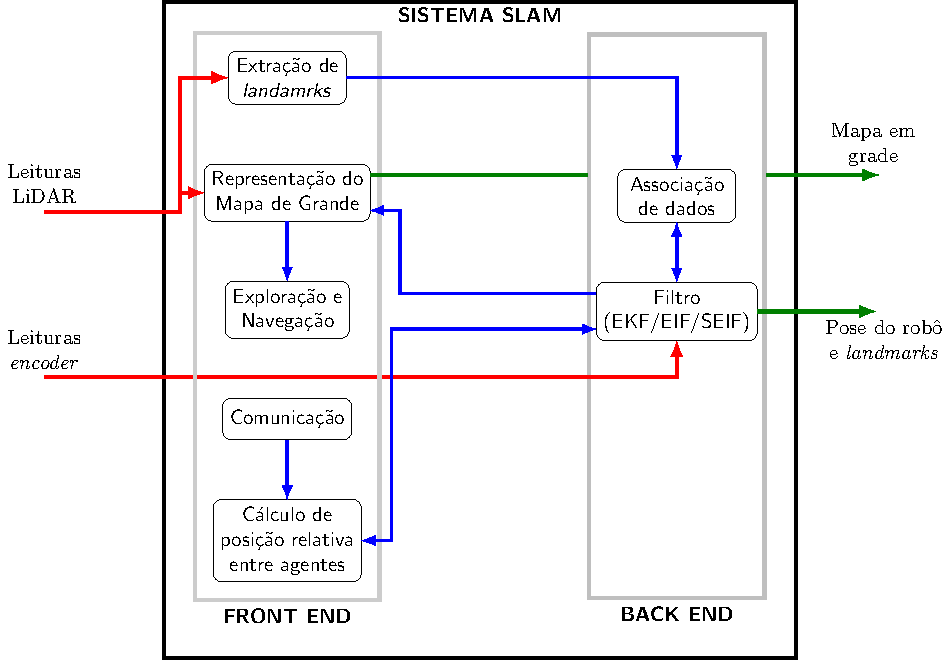
\includegraphics[width=.8\textwidth]{figs/slam-architecture.tex}
  \caption{Arquitetura simplificada do sistema SLAM desenvolvido neste trabalho. As entradas do sistema estão indicadas em vermelho, enquanto as saídas estão em verde. Em azul é 
  possível observar algumas inter relações entre módulos.}
  \label{fig:slam-architecture}
\end{figure}

\section{Organização do trabalho}
O próximo capítulo apresenta o ambiente simulado assim como o robô e os 
modelos de cinemática e medida utilizados. A organização do restante do 
trabalho é pautada pela Figura \ref{fig:slam-architecture}, o Capítulo 
3 trata da maioria dos aspectos do \textit{back-end}; começa discorrendo acerca de uma técnica clássica para resolver o problema SLAM e termina discutindo a técnica utilizada nesse trabalho; a porção do filtro responsável pela troca de mapas fica de fora desse capítulo para ser 
tratada em conjunto com a estimação de pose relativa posteriormente.

O Capítulo 4 é sobre os diversos componentes do \textit{front-end}, exceto 
a estimação de posição relativa entre os agentes. Tanto esse cálculo 
quanto a troca de mapas do \textit{back-end} são concentrados no 
Capítulo 5 por comporem a característica fundamental de 
sistemas multiagentes.

Por fim, o Capítulo 6 avalia e discute o sistema desenvolvido através de 
experimentos no ambiente simulado. O Capítulo 7, a Conclusão, sumariza 
os resultados e sugere melhorias para trabalhos futuros.